\section{Análisis de Sistemas Críticos y Tolerancia a Fallas}

Un sistema crítico (en inglés \textit{safety-critical system}) es aquel en el que un fracaso puede traer consigo consecuencias catastróficas, como daños graves a personas, pérdida de vidas o daños importantes al medio ambiente \cite[p.~271]{kopetz-2011}. Por su definición, un sistema puede caracterízarse como crítico o no crítico antes de su implementación, ya que lo que determina esto es simplemente el uso que se le dará. Algunas áreas típicas donde se pueden encontrar estos sistemas son aviónica, equipamiento médico y energía nuclear.\\

\subsection{Caso de Ejemplo: Sistema de Control de Vuelo en Aviones}

En aviónica, el sistema de control de vuelo es sin dudas un sistema crítico. Originalmente constituidos por sistemas mecánicos complejos, estos fueron reemplazados por sistemas denominados \textit{fly-by-wire}, introducidos en vuelos comerciales en el Airbus 320 en 1987 y el Boeing 777 en 1994 \cite{FBWNASA}, con el objetivo de alivianar la carga del avión y mejorar su rendimiento en cuanto al consumo de combustible. Su nombre deriva del hecho de que la acción de control del piloto no es directa sobre el avión, sino que es una computadora la que la ejecuta. Todas las señales de sensores y de comandos son transmitidas eléctricamente desde y hacia una computadora de vuelo.\\

A modo de ejemplo en la figura \ref{fig:Boeing_777_diagrama}, se muestra un diagrama simplificado de la arquitectura del sistema de control de vuelo principal del avión Boeing 777. En esta imagen se muestran distintos bloques los cuales se encuentran comunicados a través de un bus. Cuando el piloto del avión quiere ejecutar una acción, este lo hace a través de métodos convencionales como palancas o pedales que se encuentran en la cabina. Estas acciones generan señales analógicas las cuales son entregadas a los bloques denominados \textit{Actuator Control Electronics} (ACEs). Estos bloques convierten la señal analógica en una señal digital que puede enviarse a través del bus de comunicaciones a los bloques denominados \textit{Primary Flight Control System} (PFCs).

\begin{figure}[H]
    \centering
    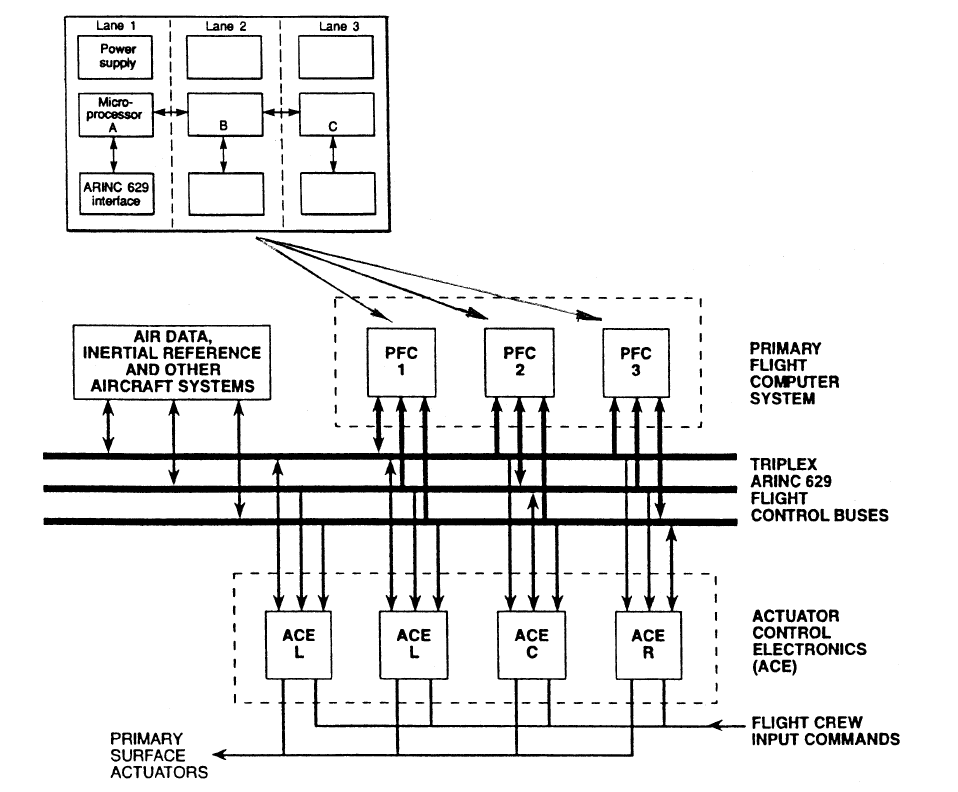
\includegraphics[width=0.7\textwidth]{img/Boeing_777_diagrama.png}
    \caption{Arquitectura del sistema principal de vuelo, conformado por varias computadoras en una configuración redundante. La imagen se extrajo de \cite{collinson2023introduction}.}
    \label{fig:Boeing_777_diagrama}
\end{figure}

Además de la acción del piloto, las PFCs toman datos de los distintos sensores para poder calcular todas las acciones de control que se aplicarán a los distintos actuadores del avión. Los resultados de los cálculos son enviados a los actuadores nuevamente a través del bus de comunicación a cada bloque ACE asignado para cada actuador el cual interpreta el comando recibido por el bus y lo convierte en una señal analógica que aplicará su actuador asignado. En \cite{yeh1996triple} puede encontrarse una explicación más detallada del funcionamiento de este sistema en el avión Boeing 777.\\

En la figura \ref{fig:Boeing_777_diagrama} lo que se observa es que hay redundancias en los bloques PFCs y ACEs. No solo eso, sino que además hay redundancias en el canal de comunicación, es decir en el bus. Por si fuera poco, en el Boeing 777, cada una de las PFCs se compone a su vez de 3 microprocesadores, cada uno con su fuente de alimentación propia e interfaz de comunicación con el bus. Cada uno de esos 3 procesadores son de distintos fabricantes y sus respectivos softwares son desarrollados por grupos de trabajo distintos. Generalmente solo un procesador de cada PFC se encuentra en funcionamiento normal y los otros actúan como monitores, verificando que lo que estas calculan es correcto.\\

Sin dudas todo el sistema de control de vuelo presenta una complejidad muy grande. El hecho de incorporar redundancias en el sistema incrementa notablemente la seguridad. La forma en la que esta se cuantifica es a través de la probabilidad de que el sistema fracase de forma catastrófica. Para aviones comerciales típicamente debe ser $10^{-9}/h$ \cite[p.~217]{collinson2023introduction}. Este valor es tan bajo que incluso es imposible de verificar de forma expermiental, ya que habría que ejecutar el sistema durante $10^9$ horas aproximadamente. La probabilidad de falla de los semiconductores no alcanza este valor \cite[p.~272]{kopetz-2011}. Este es el motivo por el cual se incluyen bloques redundantes en los sistemas de control de vuelo. Por ejemplo, el hecho de que cada PFC tenga 3 procesadores de distintos fabricantes permite eliminar problemas que sean propios del componente. A su vez, el hecho de que cada procesador tenga un software distinto desarrollado por un grupo de personas distinto permite que las fallas que estos puedan tener sean eliminadas a tiempo.\\

{\color{red} ACÁ AGREGAR UNA CUENTA SÚPER FÁCIL CON UN SISTEMA CON REDUDANCIAS EN PARALELO Y CON LA PROBABILIDAD DE FALLA EXPONENCIAL}.

El uso de redundancias trae consigo la necesidad de un sistema que administre todas las tareas de manera correcta con el objetivo de cumplir con el nivel de seguridad requerido. Por ejemplo, en el caso del Boeing 777 antes mencionado, detectar cuándo una de las PFCs llegó a un cálculo de la ley de control incorrecto, determinar si un sensor del avión dejó de funcionar y qué acción tomar en cada caso, entre otras.\\

En la figura \ref{fig:diagrama_general_fly_by_wire} se muestra un diagrama que representa de forma general la comunicación entre los distintos elementos del sistema de control de vuelo. En este se puede ver la redundancia de buses, sensores, actudaores y computadoras de vuelo.

\begin{figure}[H]
    \centering
    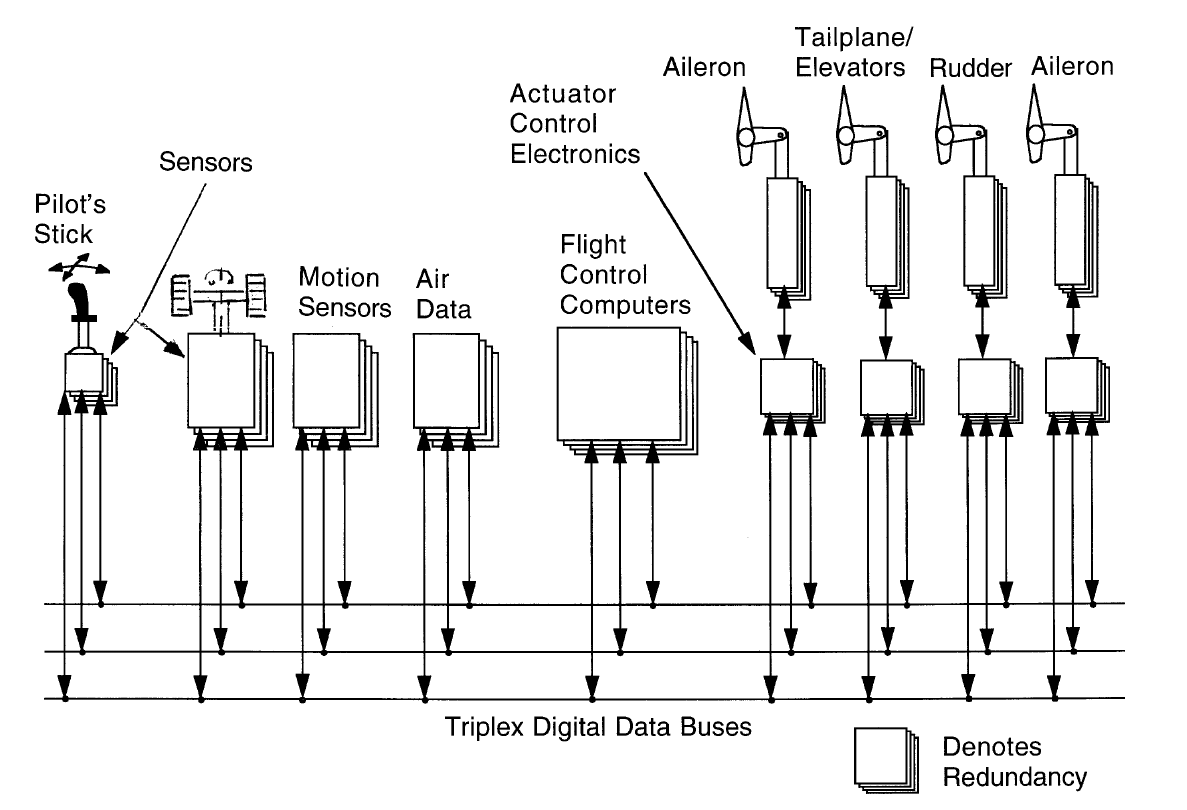
\includegraphics[width=0.8\textwidth]{img/diagrama_general_fly_by_wire.png}
    \caption{Se muestra de manera general las conexiones entre los distintos elementos del sistema de control de vuelo típico en aviones. La imagen se extrajo de \cite{collinson2023introduction}.}
    \label{fig:diagrama_general_fly_by_wire}    
\end{figure}

Cada uno de estos elementos conforman el sistema de control de vuelo tolerante a fallas en aviones. A continuación se analizan algunas de sus características.

\subsubsection{Bus de Comunicaciones}

Hasta principios de los años 70s, la comunicación entre los distintos módulos dentro de los aviones se realizaba a través de arneses de muchos cables que transmitían información en paralelo. Estos eran tan grandes que podían llegar a pesar cientos de kilogramos. Sumado a esto, la enorme cantidad de cables venía acompañada de muchas conexiones, puntos que son típicos causales de fallas intermitentes. A partir de mediados de los años 70s, se comenzó a implementar el uso de buses de comunicación serial, comunes a todos los módulos del avión. Esto simplificó muchísimo el cableado, además de facilitar el desarrollo de módulos de aviónica, ya que se simplificó la forma de comunicación con el resto del avión.\\

La comunicación serial a través del bus utiliza un acceso al medio compartido dominado por el tiempo, \textit{time-division multiple acces} (TDMA). Siguiendo con el caso del avión Boeing 777, el protocolo utilizado es el ARINC 629. Este funciona sin un nodo master y permite una conexión de hasta 120 nodos. Solamente uno de ellos puede acceder al medio físico a la vez, lo cual se define por el acceso al medio dominado por el tiempo. El medio de transmisión es un par trenzado, con una velocidad de 2 Mbit/s. A continuación, en la figura \ref{fig:ARINC_629_bus} se muestra el bus ARINC 629.

\begin{figure}[H]
    \centering
    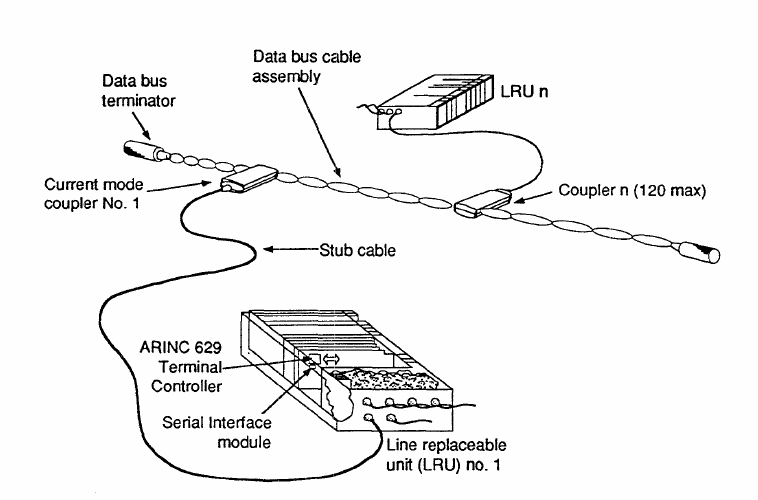
\includegraphics[width=0.7\textwidth]{img/ARINC_629_bus.png}
    \caption{Se muestra un bus ARINC 629 con 2 nodos conectados. Este consiste en un par trenzado, con terminaciones en los extremos para evitar reflexiones. La conexión de los nodos al bus no es directa si no que se utilizan acopladores. La imagen se extrajo de \cite{yeh1996triple}.}
    \label{fig:ARINC_629_bus}    
\end{figure}

El hecho de que todas las comunicaciones pasen por el mismo bus lo vuelve un punto clave en cuanto a la seguridad, ya que una falla en uno de sus cables dejaría a todos los módulos sin comunicación. Es por esto que se incluyen varios buses de estos en paralelo, como se mostró en la figura \ref{fig:diagrama_general_fly_by_wire}.\\

Un aspecto a destacar en el bus de comunicaciones es el método de acceso al medio utilizado, TDMA. El envío y recepción de mensajes se implementa por turnos. Este protocolo define en qué instantes de tiempo cada uno de los nodos puede utilizar el medio físico y en cuáles no. Para que no haya colisiones, todos los nodos deben respetar ese timing, el cual se encuentra predefinido. Esto le da determinismo y claridad al comportamiento del bus y del sistema, ya que a priori puede saberse qué mensaje se estará enviando en cada instante de tiempo. Cualquier otro tipo de comportamiento respresentará una falla. Además, al tratarse de un sistema de tiempo real, no pueden permitirse las retransmisiones, ya que es evidente que se rompería el requerimiento intrínseco de este tipo de sistemas, que es cumplir con la tarea asignada antes de cierto tiempo.

\subsubsection{Comparación de Resultados y Tolerancia a Fallas}

El mecanismo de tolerancia a fallas es a través de la comparación entre mediciones de sensores y resultados de cálculo de la ley de control. Si todos los sensores redundantes funcionan adecuadamente, es esperable que estos entreguen mediciones muy similares. Por otro lado, si uno de ellos entrega una medición diferente a la de los otros dos, se asume que este presentó una medición incorrecta. Como resultado de la comparación, se obtiene un único valor el cual es utilizado por el sistema de control. De la misma forma, se realiza una comparación de los resultados del cálculo de la ley de control obtenido por cada una de las computadoras. Una vez que se decide por un único valor, se envía la señal de acutación.\\

Existen muchos criterios utilizados para seleccionar los valores de sensores. Un aspecto importante a tener en cuenta es que a pesar de que todos los sensores redundantes funcionen adecuadamente, estos presentarán ciertas diferencias en las mediciones, algo que es esperable teniendo en cuenta cuestiones propias de la construcción de cada sensor, ruido, etc. Esto debe ser tenido en cuenta al momento de realizar las comparaciones.\\

En \cite[p.~221]{collinson2023introduction} se menciona un algoritmo muy simple. Este consiste en tomar una de las mediciones como referencia y comparar las demás contra esta. En la figura \ref{fig:votacion_sensores} se toma el ángulo $\theta_1$ como referencia, ya que $\theta_3 > \theta_1 > \theta_2$. En caso de que la diferencia $| \theta_1 - \theta_2 |$ ó $| \theta_1 - \theta_3 |$ supere un cierto límite, se asume que el sensor presentó una falla. En el caso de la imagen, la diferencia con el sensor 2 es mucho mayor que con el 3 y se asume que este presentó una falla. El valor que se toma como válido es el valor intermedio, $\theta_1$.

\begin{figure}[H]
    \centering
    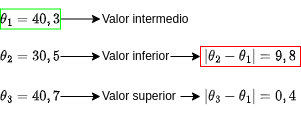
\includegraphics[width=0.5\textwidth]{img/votacion_sensores.png}
    \caption{La comparación entre 3 sensores da como resultado que el sensor 2 presentó una falla. En consecuencia deberá tomarse una acción, por ejemplo ignorar al sensor en próximas mediciones o informar al piloto.}
    \label{fig:votacion_sensores}
\end{figure}

Este mismo esquema se repite luego del cálculo de la ley de control y de los valores a aplicar sobre cada actuador.

\subsection{Comparación con Sistemas de Control de Vuelo en Drones}



\textbf{{\color{red} COMPLETAR}}